\mode*
% https://denniskubes.com/2012/08/17/basics-of-memory-addresses-in-c/
\section{Memory Model}
\begin{frame}{Memory Model}
\begin{center}
  \mode<beamer>{ 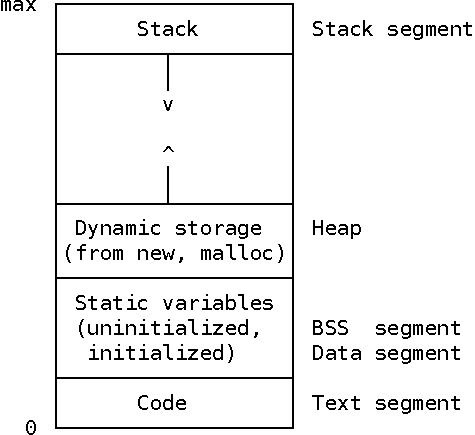
\includegraphics[width=.7\textwidth]{mem-model} }%
  \mode<article>{ 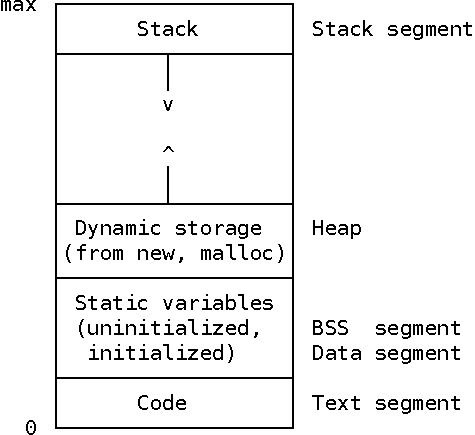
\includegraphics[width=.4\textwidth]{mem-model} }
\end{center}
\end{frame}

\begin{itemize}
\item See also: \citetitle[Sec 0x270 \emph{Memory Segmentation}]{erickson2008hacking}
\item stack setup [linux sys slides]
\item \url{http://www.dirac.org/linux/gdb/02a-Memory_Layout_And_The_Stack.php}
\item gdb (info frame, info args, info locals, ...)
\item \fxnote[inline]{make a good example using both printf() and gdb to show internals of a process}
\end{itemize}

\mode<all>
%%% Local Variables:
%%% mode: latex
%%% TeX-master: "c-b"
%%% End:
